\documentclass{beamer} %[handout]
\usetheme{CambridgeUS}
\usecolortheme{whale}
\usepackage{color}
\usepackage{xcolor}
\usepackage[makeroom]{cancel}
\usepackage{graphicx} 
\setbeamercolor{frametitle}{fg=black}
\usepackage{mathtools}
\usepackage{amssymb}
\usepackage{amsmath}
\usepackage{amsthm}
\usepackage{graphicx}
\usepackage{fancyvrb}
\usepackage{listings}
\usepackage{tikz}
\usepackage[utf8]{inputenc}

\usetikzlibrary{shapes}

\usetikzlibrary{decorations.text}

\lstset{frame=tb,
  language=R,
  aboveskip=3mm,
  belowskip=3mm,
  showstringspaces=false,
  columns=flexible,
  basicstyle={\tiny\ttfamily},
  numbers=none,
  numberstyle=\tiny\color{gray},
%  keywordstyle=\color{blue},
%  identifierstyle=\color{yellow},
  breaklines=true,
    literate={->}{$\rightarrow$}{2}
           {°}{$\epsilon$}{1},
  breakatwhitespace=true
  tabsize=3
}

\usetikzlibrary{arrows,positioning} 
\tikzset{
    %Define standard arrow tip
    >=stealth',
    %Define style for boxes
    punkt/.style={
           rectangle,
           rounded corners,
           draw=black, very thick,
           text width=6.5em,
           minimum height=2em,
           text centered},
    % Define arrow style
    pil/.style={
           ->,
           thick,
           shorten <=2pt,
           shorten >=2pt,}
}

\makeatletter
\def\th@mystyle{%
    \normalfont % body font
    \setbeamercolor{block title example}{bg=orange,fg=white}
    \setbeamercolor{block body example}{bg=orange!20,fg=black}
    \def\inserttheoremblockenv{exampleblock}
  }
\makeatother
\theoremstyle{mystyle}
\newtheorem*{remark}{Example}

\makeatletter
\def\th@mystylet{%
    \normalfont % body font
    \setbeamercolor{block title example}{bg=purple,fg=white}
    \setbeamercolor{block body example}{bg=purple!20,fg=black}
    \def\inserttheoremblockenv{exampleblock}
  }
\makeatother
\theoremstyle{mystylet}
\newtheorem*{analysis}{Example}

\date{}
\author[Bayesian statistics]{Erik \v{S}trumbelj\\2019}

\linespread{1.2}
\renewcommand{\thefootnote}{\roman{footnote}}
%\setbeameroption{show notes}

\usetikzlibrary{bayesnet}


\title[Hierarchical modelling]{Hierarchical modelling}

\begin{document}

\begin{frame}

\bigskip

\bigskip

\bigskip

\centering

\includegraphics[width=0.90\linewidth]{../LectureAssets/L07/Lecture07cartoon}

\bigskip

\end{frame}

\begin{frame}
Bayesian statistics
\titlepage
\end{frame}


\begin{frame}{Outline}

\begin{itemize}\itemsep1.5em

\item \textbf{Plate notation} - DAGs and Bayesian networks.

\item  \textbf{Hierarchical modelling} - multilevel/mixed-effects modelling the Bayesian way.

\item  Bayesian interpretation of \textbf{regularization} and corrections for \textbf{multiple hypothesis testing}.

\item  Unrelated: \textbf{mixture modelling}.

\end{itemize}
\end{frame}

\begin{frame}{Directed Acyclic Graph (DAG)}

\begin{small}
\textbf{Directed Acyclic Graph} (DAG) is a directed simple graph without cycles.

\bigskip



\begin{minipage}[c]{0.47\linewidth}
DAG:

\centering
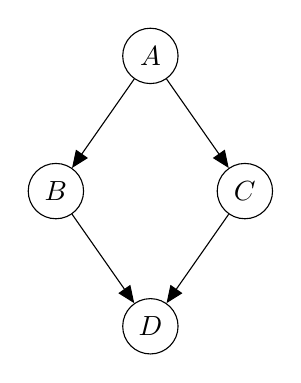
\begin{tikzpicture}

  % Define nodes
  \node[latent]                               (d) {$D$};
  \node[latent, above=of d, xshift=-1.2cm] (b) {$B$};
  \node[latent, above=of d, xshift=1.2cm]  (c) {$C$};
  \node[latent, above=of b, xshift=1.2cm]            (a) {$A$};

  % Connect the nodes
  \edge {b,c} {d} ; %
  \edge {a} {b,c} ; %
\end{tikzpicture}
\end{minipage}
\begin{minipage}[c]{0.47\linewidth}
Not a DAG:

\centering
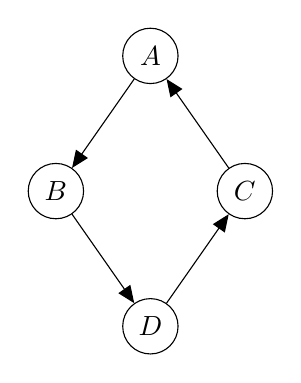
\begin{tikzpicture}

  % Define nodes
  \node[latent]                               (d) {$D$};
  \node[latent, above=of d, xshift=-1.2cm] (b) {$B$};
  \node[latent, above=of d, xshift=1.2cm]  (c) {$C$};
  \node[latent, above=of b, xshift=1.2cm]            (a) {$A$};

  % Connect the nodes
  \edge {b} {d} ; %
  \edge {a} {b} ; %
    \edge {d} {c} ; %
  \edge {c} {a} ; %
\end{tikzpicture}
\end{minipage}
\bigskip

DAGs are a very useful representation of dependencies (and conditional independencies) between random variables in a Bayesian model.

\bigskip

Model can be represented with a DAG $\Leftrightarrow$ Model is a \textbf{Bayesian network}.
\end{small}
\end{frame}



\begin{frame}{Plate notation}

Simplifying repetitions with a plate:
\begin{center}
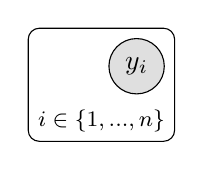
\begin{tikzpicture}
  \node[obs](y){$y_i$};
  \plate {} {(y)} {$i \in \{1,...,n\}$}; %
\end{tikzpicture}
\end{center}

\smallskip

Plate notation sometimes features additional information:

\bigskip

\begin{scriptsize}

\begin{minipage}[c]{0.45\linewidth}
Latent variable:
\smallskip 
\begin{center}
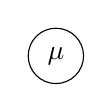
\begin{tikzpicture}
  \node[latent](a){$\mu$};
\end{tikzpicture}
\end{center}

Data:
\smallskip
\begin{center}
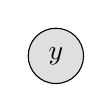
\begin{tikzpicture}
\node[obs] (a) {$y$};
\end{tikzpicture}
\end{center}
\end{minipage}
\begin{minipage}[c]{0.45\linewidth}
Deterministic node:
\smallskip 
\begin{center}
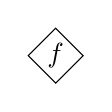
\begin{tikzpicture}
  \node[det](a){$f$};
\end{tikzpicture}
\end{center}
Constant:
\smallskip 
\begin{center}
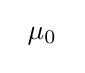
\begin{tikzpicture}
  \node[const](a){$\mu_0$};
\end{tikzpicture}
\end{center}
\end{minipage}
\end{scriptsize}
\smallskip


\end{frame}


\begin{frame}{DAG-based factorization of the joint distribution}

Take the joint distribution $ p(\theta_1, \theta_2, \dots, \theta_n)$ and a DAG that represents (in)dependencies between $\theta_i$.

\bigskip

The joint distribution factorizes:

$$ p(\theta_1, \theta_2, \dots, \theta_n) = \prod_{i=1}^n p\left(\theta_i|\text{parents}(\theta_i)\right).$$

\end{frame}


\begin{frame}{Factorizing full-conditionals}

\begin{small}

Given a DAG representation, the joint posterior of parameters $\theta$ factorizes:

$$ p(\theta | y) = \frac{p(\theta, y)}{p(y)} \propto p( \theta, y) = p(V) = \prod_{v \in V} p\left(v|\text{parents}(v)\right).$$

\bigskip

\bigskip

Full-conditional for parameter $\theta_i$:

$$p(\theta_i | V \setminus \theta_i) = \frac{p(V)}{p(V\setminus \theta_i)} \propto P(V) \propto p(\theta_i|\text{parents}(\theta_i)) \prod_{w \in \text{children}(\theta_i)}  p(w|\text{parents}(w))$$
\end{small}
\end{frame}


\begin{frame}{Sampling hierarchy used by software}

\begin{small}
\bigskip

$$p(\theta_i | y, \theta_{-i}) \propto p(\theta_i|\text{parents}(\theta_i)) \prod_{w \in \text{children}(\theta_i)}  p(w|\text{parents}(w))$$

\bigskip
\end{small}

We can automatically derive and evaluate the full-conditionals. Additionally, we have a symbolic representation of their shapes.

\bigskip

We can use this information to select more efficient sampling than M-H for each individual full-conditional.

\bigskip


\begin{center}
\includegraphics[scale=.37]{../LectureAssets/L07/WinBugsHierarchy}
\end{center}
\bigskip

\end{frame}


\begin{frame}{1st generation Bayesian inference software}

\bigskip

\textbf{Input: }Model description (in software's modelling language) \& data.

\bigskip

\begin{itemize}\itemsep1.1em
\item Deduce DAG from model description.
\item Factorize full-conditionals based on DAG.
\item Recognize conjugacy, etc... and select most efficient sampling for each parameter.
\item Gibbs sampling.
\end{itemize}

\bigskip

\textbf{Output:} MCMC samples from posterior.

\bigskip

Representatives: BUGS, WinBUGS, OpenBUGS, JAGS.

\end{frame}

\begin{frame}{A hierarchical model for the means of groups}
\smallskip

\begin{columns}[c]
\centering
\column{.40\textwidth}
$ Y_{ij} \sim N(\mu_j, \sigma^2)$, 

$ \mu_j \sim N(\mu_{\mu}, \sigma_{\mu}^2)$, 

$ \sigma^2 \sim IG(a, b)$,

$ \mu_{\mu} \sim N(\mu_0, \sigma^2_0)$, 

$ \sigma_{\mu}^2 \sim IG(a,b)$.

\column{.60\textwidth}

Plate notation:

\begin{center}
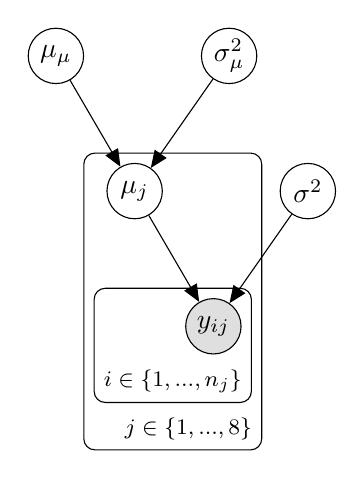
\begin{tikzpicture}
\node[obs] (y3) {$y_{ij}$};
\node[latent, above=of y3, xshift = 1.2cm] (t2) {$\sigma^2$};
\node[latent, above=of y3, xshift = -1.0cm] (t1) {$\mu_j$};
\node[latent, above=of t1, xshift = 1.2cm] (tt2) {$\sigma_{\mu}^2$};
\node[latent, above=of t1, xshift = -1.0cm] (tt1) {$\mu_{\mu}$};
\edge {t1,t2} {y3} ; %
\edge {tt1,tt2} {t1} ; %

  \plate {p1} {(y3)} {$i \in \{1,...,n_j\}$}; %
  \plate {} {(y3)(t1)(p1)} {$j \in \{1,...,8\}$}; %
  
\end{tikzpicture}
\end{center}
\end{columns}
\end{frame}


\begin{frame}[fragile]{JAGS example}
\smallskip

\begin{columns}[c]
\centering
\column{.40\textwidth}
$ Y_{ij} \sim N(\mu_j, \sigma^2)$, 

$ \mu_j \sim N(\mu_{\mu}, \sigma_{\mu}^2)$, 

$ \sigma^2 \sim IG(10^{-4}, 10^{-4})$,

$ \mu_{\mu} \sim N(0, 10^6)$, 

$ \sigma_{\mu}^2 \sim IG(10^{-4}, 10^{-4})$.

\column{.60\textwidth}

JAGS:

\begin{center}
\begin{scriptsize}
\begin{lstlisting}[language=R, frame=leftline]
model {
  tau ~ dgamma(0.001, 0.001) 
  tauMu ~ dgamma(0.001, 0.001)
  muMu ~ dnorm(0,1/100)

  for (j in 1:k) {
    mu[j] ~ dnorm(muMu, tauMu)
    for (i in 1:n[j]) {
      y[j,i] ~ dnorm(mu[j], tau)
    }
  }
 
  sigma2 <- 1 / tau
  sigma2mu <- 1 / tauMu
}
\end{lstlisting}
\end{scriptsize}
\end{center}
\end{columns}
\end{frame}

\begin{frame}
\begin{analysis}[Estimating piglet weight for multiple litters]

\smallskip

\begin{minipage}[c]{0.33\linewidth}
\includegraphics[width=1.0\linewidth]{../LectureAssets/L07/piglets}
\end{minipage} 
\begin{minipage}[r]{0.65\linewidth}
\begin{center}
\begin{tiny}
\tabcolsep=0.11cm
\begin{tabular}{rrrrrrrr}
  \hline
 i=1 & i=2 & i=3 & i=4 & i=5 & i=6 & i=7 & i=8 \\ 
  \hline
  2.0 & 3.5 & 3.3 & 3.2 & 2.6 & 3.1 & 2.6 & 2.5 \\ 
  2.8 & 2.8 & 3.6 & 3.3 & 2.6 & 2.9 & 2.2 & 2.4 \\ 
  3.3 & 3.2 & 2.6 & 3.2 & 2.9 & 3.1 & 2.2 & 3.0 \\ 
  3.2 & 3.5 & 3.1 & 2.9 & 2.0 & 2.5 & 2.5 & 1.5 \\ 
  4.4 & 2.3 & 3.2 & 3.3 & 2.0 &  & 1.2 &  \\ 
  3.6 & 2.4 & 3.3 & 2.5 & 2.1 &  & 1.2 &  \\ 
  1.9 & 2.0 & 2.9 & 2.6 &  &  &  &  \\ 
  3.3 & 1.6 & 3.4 & 2.8 &  &  &  &  \\ 
  2.8 &  & 3.2 &  &  &  &  &  \\ 
  1.1 &  & 3.2 &  &  &  &  &  \\ 
  \hline
  2.84 & 2.66 & 3.18 & 2.98 & 2.37 & 2.90&  1.98 & 2.35  \\
  
   \hline
   \hline
\end{tabular}
\end{tiny}
\end{center}
\end{minipage}

\bigskip

We are interested in estimating/comparing expected piglet weight for several litters, each litter from a different pig.

\bigskip

\bigskip

\end{analysis}
\end{frame}



\begin{frame}
\begin{analysis}[Estimating piglet weight for multiple litters]

\bigskip

\textbf{Model suggestion 1:}

\bigskip

\smallskip

$ y_i \sim N(\mu, \sigma^2)$, $ \mu \sim N(\mu_0, \sigma_0^2)$, $ \sigma^2 \sim IG(\alpha_0, \beta_0).$

\bigskip

\bigskip

\begin{center}
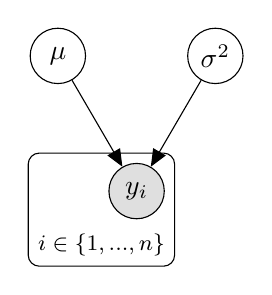
\begin{tikzpicture}
\node[obs] (y3) {$y_i$};
\node[latent, above=of y3, xshift = 1.0cm] (t2) {$\sigma^2$};
\node[latent, above=of y3, xshift = -1.0cm] (t1) {$\mu$};
\edge {t1,t2} {y3} ; %
  \plate {} {(y3)} {$i \in \{1,...,n\}$}; %
\end{tikzpicture}
\end{center}

\smallskip

\end{analysis}
\end{frame}

\begin{frame}
\begin{analysis}[Estimating piglet weight for multiple litters]

\bigskip

\textbf{Model suggestion 2:}

\bigskip

\smallskip

$ y_{i,j} \sim N(\mu_j, \sigma^2)$, $ \mu_j \sim N(\mu_0, \sigma_0^2)$, $ \sigma^2 \sim IG(\alpha_0, \beta_0).$

\bigskip

\bigskip

\begin{center}
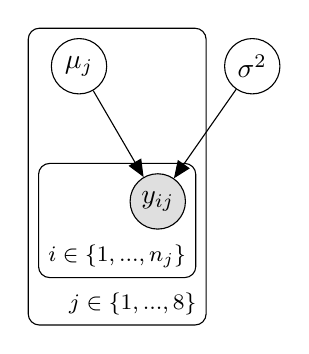
\begin{tikzpicture}
\node[obs] (y3) {$y_{ij}$};
\node[latent, above=of y3, xshift = 1.2cm] (t2) {$\sigma^2$};
\node[latent, above=of y3, xshift = -1.0cm] (t1) {$\mu_j$};
\edge {t1,t2} {y3} ; %
  \plate {p1} {(y3)} {$i \in \{1,...,n_j\}$}; %
  \plate {} {(y3)(t1)(p1)} {$j \in \{1,...,8\}$}; %
  
\end{tikzpicture}
\end{center}

\smallskip

\end{analysis}
\end{frame}


\begin{frame}
\begin{analysis}[Estimating piglet weight for multiple litters]

\bigskip

\textbf{Model suggestion 3:}

\bigskip

\begin{columns}[c]
\centering
\column{.40\textwidth}
$ Y_{ij} \sim N(\mu_j, \sigma^2)$, 

$ \mu_j \sim N(\mu_{\mu}, \sigma_{\mu}^2)$, 

$ \sigma^2 \sim IG(a_0, b_0)$,

$ \mu_{\mu} \sim N(\mu_0, \sigma^2_0)$, 

$ \sigma_{\mu}^2 \sim IG(a_0,b_0)$.

\column{.60\textwidth}

\begin{center}
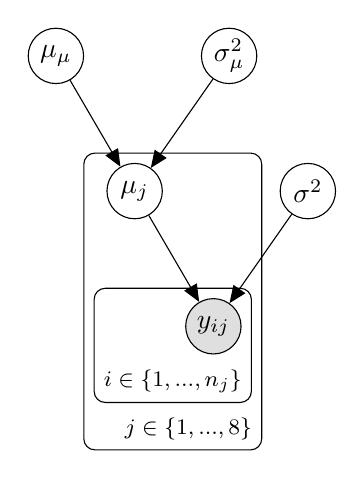
\begin{tikzpicture}
\node[obs] (y3) {$y_{ij}$};
\node[latent, above=of y3, xshift = 1.2cm] (t2) {$\sigma^2$};
\node[latent, above=of y3, xshift = -1.0cm] (t1) {$\mu_j$};
\node[latent, above=of t1, xshift = 1.2cm] (tt2) {$\sigma_{\mu}^2$};
\node[latent, above=of t1, xshift = -1.0cm] (tt1) {$\mu_{\mu}$};
\edge {t1,t2} {y3} ; %
\edge {tt1,tt2} {t1} ; %

  \plate {p1} {(y3)} {$i \in \{1,...,n_j\}$}; %
  \plate {} {(y3)(t1)(p1)} {$j \in \{1,...,8\}$}; %
  
\end{tikzpicture}
\end{center}
\end{columns}

\smallskip

\end{analysis}
\end{frame}


\begin{frame}{Hierarchical (multi-level) models}

In practice, we often deal with data from different but similar groups and the models we use should reflect this.

\bigskip

The Bayesian approach to this is to put priors on priors (hyper-priors), resulting in a hierarchical (multi-level) structure of the model.

\bigskip

A hierarchical structure also lets us use more parameters (a more complex model) without overfitting!

\bigskip

Hierarchical models are the quintessential Bayesian approach:
\begin{itemize}
\item Group comparison.
\item Correction for testing multiple hypotheses.
\item Regularizaton.
\item ...
\end{itemize}

\end{frame}


\begin{frame}
\begin{analysis}[Estimating piglet weight for multiple litters]

\bigskip

\begin{center}
\includegraphics[scale=0.5]{../LectureAssets/L07/piglets_compare}
\end{center}
\smallskip

\begin{small}
Estimate shrinkage: Same principles alleviate issues with multiple comparisons.

\bigskip
\end{small}

\end{analysis}
\end{frame}


\begin{frame}
\begin{analysis}[Ozone concentration forecasting]
\bigskip

\begin{center}
\includegraphics[scale=0.35]{../LectureAssets/L07/pollution}
\end{center}

Task: One-day-ahead forecasting of O$_3$ concentration from 100s of meteorological, pollution-related, and other input variables.
\end{analysis}
\end{frame}


\begin{frame}
\begin{analysis}[Ozone concentration forecasting - Prediction quality]
\bigskip

\bigskip
\begin{center}
\includegraphics[scale=0.47]{../LectureAssets/L07/ozone_MSE}
\end{center}

\smallskip
\end{analysis}
\end{frame}

\begin{frame}
\begin{analysis}[Ozone concentration forecasting - Coefficients]
\smallskip
\begin{center}
\includegraphics[scale=0.47]{../LectureAssets/L07/ozone_coeff}
\end{center}

\end{analysis}
\end{frame}

\begin{frame}
\begin{analysis}[Fitting multimodal densities]

\bigskip

\bigskip

\begin{center}
\includegraphics[width=0.70\linewidth]{../LectureAssets/L07/fmDataset}
\end{center}

\bigskip

\end{analysis}
\end{frame}

\begin{frame}[fragile]
\begin{analysis}[A k-component finite Normal mixture model]

{\fontsize{5}{5} \selectfont
\begin{center}
\begin{verbatim}
data {
  int<lower=1> K; // number of mixture components
  int<lower=1> N;
  real y[N];
}

parameters {
  simplex[K] theta;       // mixing proportions
  real mu[K];             // locations of mixture components
  real<lower=0> sigma[K]; // scales of mixture components
}

model {
  real ps[K];              // temp for log component densities
  sigma ~ cauchy(0,2.5);
  mu ~ normal(0,10);
  
  for (n in 1:N) {
    for (k in 1:K) {
      ps[k] = log(theta[k]) + normal_lpdf(y[n] | mu[k], sigma[k]);
    } 
    target += log_sum_exp(ps);
  }
}

generated quantities {
// only goal is for the model to output the log-likelihood
  real ps[K];
  real log_lik[N];
  for (n in 1:N) {
    for (k in 1:K) {
         ps[k] = log(theta[k]) + normal_lpdf(y[n] | mu[k], sigma[k]);
    }
  
    log_lik[n] = log_sum_exp(ps);
  }
}
\end{verbatim}
\end{center}}

\end{analysis}
\end{frame}

\begin{frame}
\begin{analysis}[K=1]

\smallskip

A few samples from the posterior:

\smallskip

\begin{center}
\includegraphics[width=0.70\linewidth]{../LectureAssets/L07/fm_fit01}
\end{center}

\bigskip

\end{analysis}
\end{frame}

\begin{frame}
\begin{analysis}[K=2]

\smallskip

Traceplot (5 chains):

\smallskip

\begin{center}
\includegraphics[width=0.90\linewidth]{../LectureAssets/L07/fm_traceplot02}
\end{center}

\smallskip

\end{analysis}
\end{frame}


\begin{frame}[fragile]
\begin{analysis}[K=2]

\smallskip

Summary (5 chains):

\smallskip

\begin{tiny}

\begin{verbatim}
                  mean se_mean   sd     2.5%      25%      50%      75%    97.5% n_eff  Rhat
theta[1]          0.54    0.12 0.19     0.28     0.31     0.68     0.70     0.73     3 12.13
theta[2]          0.46    0.12 0.19     0.27     0.30     0.32     0.69     0.72     3 12.13
mu[1]             0.17    0.91 1.43    -1.04    -1.00    -0.98     1.90     2.05     3 26.04
mu[2]             0.75    0.90 1.43    -1.03    -0.99     1.83     1.94     2.06     3 21.62
sigma[1]          0.74    0.17 0.27     0.49     0.52     0.54     1.04     1.18     3  6.44
sigma[2]          0.85    0.17 0.28     0.49     0.53     1.01     1.08     1.20     3  5.41
ps[1]            -4.60    2.04 3.27    -9.95    -8.18    -2.05    -1.96    -1.84     3  5.82
ps[2]            -5.86    2.02 3.25   -10.05    -8.65    -7.51    -1.99    -1.86     3  4.80
\end{verbatim}
\smallskip
\end{tiny}

\end{analysis}
\end{frame}


\begin{frame}
\begin{analysis}[K=2]

\smallskip

A few samples from the posterior:

\smallskip

\begin{center}
\includegraphics[width=0.70\linewidth]{../LectureAssets/L07/fm_fit02}
\end{center}

\bigskip

\end{analysis}
\end{frame}

\begin{frame}[fragile]
\begin{analysis}[Model quality]

\bigskip

\begin{verbatim}
MSE:
         Estimate    SE
model1       2.32  0.10
model2       3.09  0.18
\end{verbatim}\pause

\begin{verbatim}
looic (approximate LOOCV log score):
         Estimate    SE
model1     3684.1  45.3
model2     3049.1  57.2
\end{verbatim}

\bigskip

\end{analysis}
\end{frame}

\end{document}
